\chapter{Architetture di Base}
\section{Moduli moltiplicativi}
Iniziamo in primis da delle architetture molto semplici che useremo molte volte all'interno del corso, esse sono i moduli moltiplicativi. Possiamo notare come si può effettuare il processo di backpropagation rispetto agli input, ma anche rispetto a dei pesi. Pertanto ci chiediamo qual è la differenza fra gli input e i pesi, la prima che ci viene in mente senz'altro è quella che i primi non sono direttamente imparabili, gli altri invece no. Ma cosa succederebbe nel caso in cui i pesi fossero gli output di un'altra Neural Network ? Questa possibilità risulta essere possibile e viene effettuata molto spesso in Deep Learning.

\begin{equation}
    s_i = \sum_{j}w_{ij}x_{j}\,:\, w_{ij}=\sum_ku_{ijk}z_k \Rightarrow s_i=\sum_{jk}u_{ijk}z_kx_j
    \label{eq:weightAsInput}
\end{equation}

\begin{figure}
    \centering
    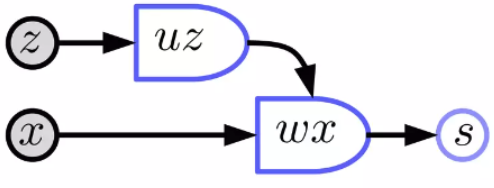
\includegraphics[width=0.3\linewidth]{figure/WeightAsInput.png}
    \caption{Grafo computazionale corrispettivo all'equazione~\ref{eq:weightAsInput}}
    \label{fig:wai}
\end{figure}

Viene pertanto automatico chiedersi, nel caso in cui avessimo una Neural Network che controlla i pesi, siamo in grado di ricrearne una nuova, modificandone soltanto i pesi, o combinando gli output. Questa cosa risulta essere possibile, e una singola Neural Network è in grado di controllarne altre due, potremmo tuttavia avere dei limiti i quali dobbiamo imporre nella nostra equazione. Inanzitutto, dobbiamo evitare che i numeri delle reti neurali possano portare a generare un'esplosione di alcune delle nuove reti. Quello che vogliamo pertanto, è che la somma dei differenti pesi sia controllata dalla nostra prima rete neurale, facendi si, che sia in grado di decidere quali reti neurali vogliamo che si attivino e quali no, si può vedere matematicamente dall'equazione~\ref{eq:attentionMod}. È un meccanismo facilmente implementabile utilizzando un modulo chiamato \textit{SoftMax}, sul quale ci soffermeremo più avanti, esso ci permette di calcolare nuovi pesi oltre all'attivazione. Questa tipologia di architettura, in cui abbiamo una rete la quale controlla altre reti, prende il nome di \textbf{Modulo dell'attenzione}, chiamato così perché, in base agli input decide di dare più o meno importanza alle singole reti neurali.

\begin{equation}
    s_i = \sum_jw_jx_{ij} \,:\,w_j=\frac{e^{z_{j}}}{\sum_ke^{z_k}}
    \label{eq:attentionMod}
\end{equation}

\begin{figure}
    \centering
    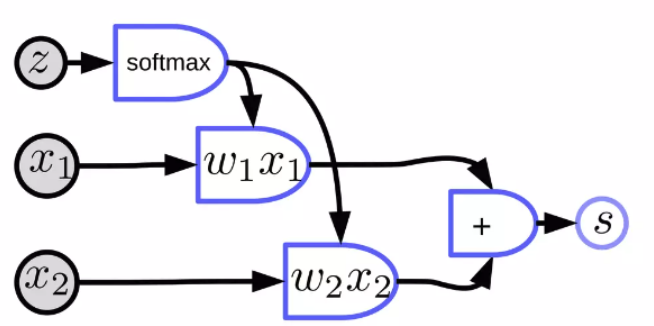
\includegraphics[width=0.35\linewidth]{figure/AttentionModule.png}
    \caption{Grafo computazionale del controllo effettuato su nuove rete neurali generate da una prima}
    \label{fig:AttentionMod}
\end{figure}

Possiamo immaginare questi moduli moltiplicativi in una maniera dettagliata, vogliano utilizzare una risorsa esterna per attivare e disattivare un input che potrebbe essere inserito in un'altra rete neurale, come se stessimo parlando di uno switch. La modalità più efficace per far ciò, è usare come moltiplicatori 0 e 1, facendo si che se immettessi 1 e 0 attiverò una parte del mio modulo, mentre se immettessi 0 e 1 attiverò l'altra. Tuttavia giunti a questo punto vi è un problema, ossia 1 e 0 sono dei numeri, e non possiamo differenziare rispetto a dei numeri, ma se sostituissimo questi valori con gli output di un'altra rete neurale, la backpropagation potrebbe essere effettuata.

\subsubsection{Mixture of Experts}
Fondamentalmente l'idea che stiamo analizzando inserendo più reti neurali in un'unica architettura, prende il nome di \textbf{Mixture of Experts}, infatti partendo da una semplice rete neurale con $x_1$ e $x_2$ come ingressi, l'abbiamo estesa sempre più rendendola ma estendendola diventando un'\textit{esperta}, creando una rete neurale molto grande con all'interno milioni e milioni di parametri, come per esempio possiamo immaginarci un modello di linguaggio. Il modello Mixture of Experts, è una rete neurale, la quale ci permette di selezionare su quale modello specifico fare affidamento per compiere un determinato task (Figura~\ref{fig:mixExp}). Alcuni dei più utilizzati modelli di linguaggio infatti prendono in considerazione una combinazione di esperti specializzati in attività specifiche (es. Traduzione, riassunto, calcoli, ecc\dots). 

\begin{figure}
    \centering
    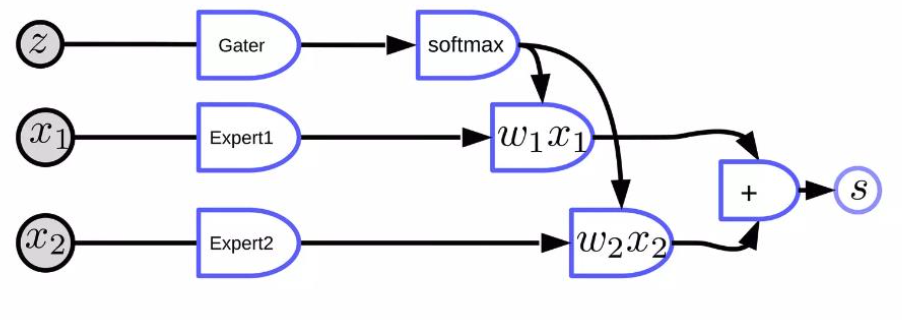
\includegraphics[width=0.50\linewidth]{figure/MixtureOfExpert.png}
    \caption{Grafo computazionale, rappresentativo di un modello di Mixture of Experts, un mix di modelli esperti in compiti specifici attivati o disattivati da un'altra rete neurale tramite l'utilizzo della funzione softmax.}
    \label{fig:mixExp}
\end{figure}

\subsubsection{Parameter Transoformation}
Possiamo vedere l'operazione generata da un'architettura di Mixture of Experts, in un'altra maniera, ci basti immaginare un parametro W, il quale viene utilizzato in una rete per venire trasformato, chiamiamo infatti questa operazione: \textbf{Parameter Trasformation}. Questa procedura risulta essere molto importante, poiché possiamo avere diverse modalità di trasformazioni sui parametri, una di queste è la \textbf{Condivisione dei pesi}. La condivisione dei pesi è una tecnica in cui lo stesso insieme di parametri viene utilizzato più volte in diverse parti del modello, riducendo il numero totale di parametri e migliorandone l'efficienza complessiva. Si può considerare come un blocco il quale a un singolo input assegna più output, dove questi output sono pesi diversi, venendo poi inseriti nella nostra rete neurale principale. Questa tecnica la possiamo utilizzare in diverse parti del nostro input, ottenendo poi diverse funzioni di costo che possono essere combinate. Dunque, modificheremo questa rete, attraverso la backpropagation la quale ci permetterà di ottenere nuovi pesi che funzioneranno per tutti i possibili input, creando un modello capace di generallizare meglio di prima (Figura~\ref{fig:wshar}).

\begin{figure}
    \centering
    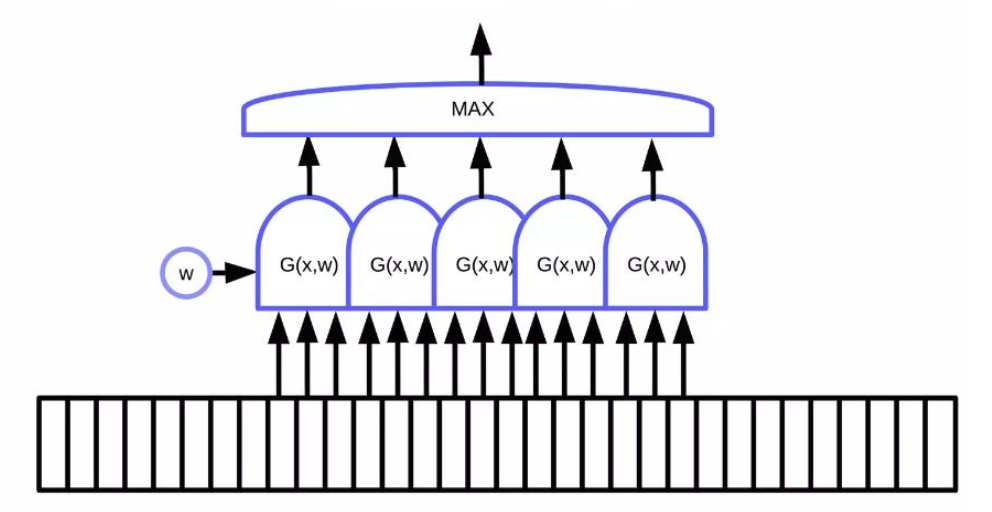
\includegraphics[width=0.50\linewidth]{figure/WeightShar.png}
    \caption{Grafo computazionale che sintetizza la condivisione dei pesi, utilizzandoli come input differenti generando nuove funzioni di costo, permettendo di generalizzare il modello su diversi input.}
    \label{fig:wshar}
\end{figure}